28. $f(x)=\cfrac{x+2-|2x+1|}{x^2-1}=\begin{cases}\cfrac{-x+1}{(x-1)(x+1)},\ x\geqslant-\cfrac{1}{2},\\ \cfrac{3x+3}{(x-1)(x+1)},\ x<-\cfrac{1}{2}.\end{cases}=
\begin{cases}-\cfrac{1}{x+1},\ x\geqslant-\cfrac{1}{2},\ x\neq1,\\ \cfrac{3}{x-1},\ x<-\cfrac{1}{2},\ x\neq-1.\end{cases}$
$$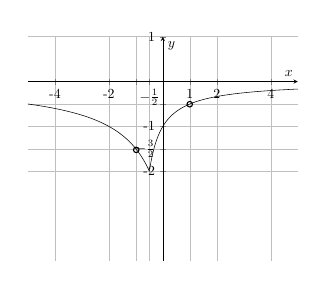
\begin{tikzpicture}[scale=0.5]
\begin{axis}[
    axis lines = middle,
    grid=major,
    legend pos={south west},
    xlabel = {$x$},
    %xlabel style={below right},
    ylabel = {$y$},
    ymin=-4,
    ymax=1,
    xtick={-4, -2,-1,-0.5,1, 2,4},
    xticklabels={-4, -2,$ $,$-\frac{1}{2}$, 1, 2, 4},
    ytick={-2,-1.5,-1,-0.5, 1, 2},
     yticklabels={-2,$-\frac{3}{2}$,-1,$ $, 1, 2},
                  ]
	\addplot[domain=-5:-0.5, samples=100, color=black] {3/(x-1)};
    %\addplot[domain=-0.99:0.5, samples=100, color=black] {1/(1-x)};
    \addplot[domain=-0.5:5, samples=100, color=black] {-1/(x+1)};
   % \addplot[domain=1.01:5, samples=100, color=black] {3/(x+1)};
    %\addlegendentry{$\text{Рис. 1}$};
\end{axis}
\draw (2.75,2.82) circle (2pt);
\draw (4.11,3.98) circle (2pt);
\end{tikzpicture}$$
б) По графику определим $D(f)=(-\infty;-1)\cup(-1;1)\cup(1;+\infty),\ E(f)=[-2;0).$\\
в) По графику определим количесво решений: $a\in(-\infty;-2)\cup[0;+\infty):0,\ a\in\left\{-2;-\cfrac{3}{2}; -\cfrac{1}{2}\right\}:1,$\\$ a\in\left(-2;-\cfrac{3}{2}\right)\cup\left(-\cfrac{3}{2};-\cfrac{1}{2}\right)\cup\left(-\cfrac{1}{2};0\right):2.$\\
